%%=============================================================================
%% Methodologie
%%=============================================================================

\chapter{\IfLanguageName{dutch}{Methodologie}{Methodology}}
\label{ch:methodologie}

%% TODO: Hoe ben je te werk gegaan? Verdeel je onderzoek in grote fasen, en
%% licht in elke fase toe welke stappen je gevolgd hebt. Verantwoord waarom je
%% op deze manier te werk gegaan bent. Je moet kunnen aantonen dat je de best
%% mogelijke manier toegepast hebt om een antwoord te vinden op de
%% onderzoeksvraag.

Om tot een correct mogelijk resultaat te komen is het belangrijk om een grondige kennis te hebben van de geïmplementeerde algoritmen, modellen en platformen. Die zijn samen gebundeld tot een huidige stand van zaken en zijn terug te vinden in hoofdstuk \ref{ch:stand-van-zaken}.

Er worden meerdere \textit{cases} opgezet die telkens volgens dezelfde criteria gequoteerd worden. Verdere informatie over de gebruikte datasets is beschreven in sectie \ref{sec:datasets}. De vereisten waaraan elk systeem zo veel mogelijk aan moet voldoen worden toegelicht aan de hand van een requirements analyse in sectie \ref{sec:requirements}.

Het hoofddoel van dit onderzoek is ontdekken als de huidige staat van de technologie bruikbaar is in een bedrijfscontext zonder extreme operationele veranderingen. Dit kan afhangen van kosten om het systeem te gebruiken, extra mankracht die nodig is, eventuele omscholing enzovoort. De conclusie zal rond die vereisten geformuleerd worden. Omdat er verschillende implementaties getest worden is het ook een vergelijkende studies en moeten ze onderling tegen elkaar geëvalueerd worden. Dit niet alleen vanuit een technologisch standpunt (wat onderzocht wordt in deze studie) maar ook de bijdrage die het levert aan de \textit{business value}. Om dit zo correct mogelijk te doen wordt in de achtergrond van de conclusie rekening gehouden met resultaten uit een studie vanuit een economisch standpunt. 

\section{Datasets}
\label{sec:datasets}

De keuze van de dataset is belangrijk. Dit onderzoek wil de capaciteiten van AutoML systemen testen op realistische situaties. De traditionele datasets (CIFAR, MNIST ...) waarmee deze algoritmen getraind zijn vallen onmiddellijk uit de selectie zoals uitgelegd in sectie \ref{subsec:autokeras}.

\subsection{Cats vs dogs}
\label{subsec:catsvsdogs}

\begin{figure}
    \begin{subfigure}{.5\textwidth}
        \centering
        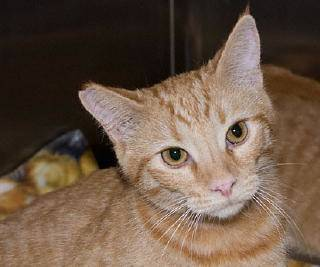
\includegraphics[width=.8\linewidth]{img/good_cat.jpg}
        \label{fig:cat-goog}
    \end{subfigure}%
    \begin{subfigure}{.5\textwidth}
        \centering
        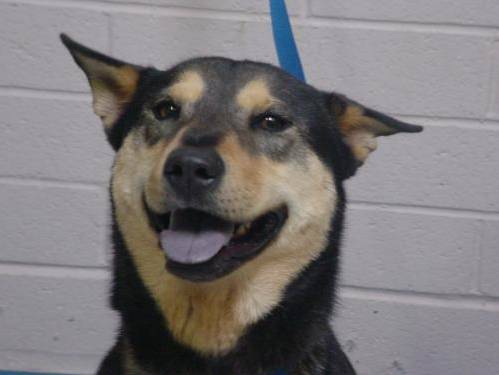
\includegraphics[width=.8\linewidth]{img/good_dog.jpg}
        \label{fig:dog-good}
    \end{subfigure}
    \caption{Kat en hond zijn de focus van de afbeelding.}
    \label{fig:catdog-good}
\end{figure}

\begin{figure}
    \begin{subfigure}{.5\textwidth}
        \centering
        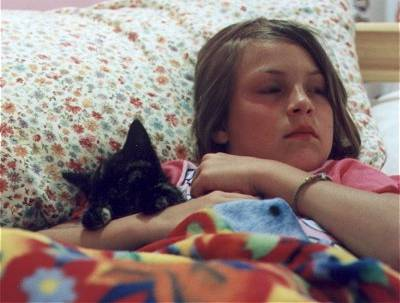
\includegraphics[width=.8\linewidth]{img/bad_cat.jpg}
        \label{fig:cat-bad}
    \end{subfigure}%
    \begin{subfigure}{.5\textwidth}
        \centering
        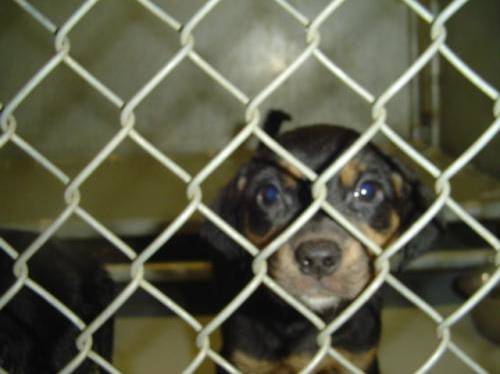
\includegraphics[width=.8\linewidth]{img/bad_dog.jpg}
        \label{fig:dog-bad}
    \end{subfigure}
    \caption{Kat en hond zijn niet de focus van de afbeelding.}
    \label{fig:catdog-bad}
\end{figure}

Een eerste testronde wordt uitgevoerd met een online\footnote{\url{https://www.kaggle.com/c/dogs-vs-cats/data}} dataset over katten en honden. Ooit was de dataset het onderwerp van een \textit{data science} wedstrijd en mogen vrij gebruikt worden. Ze bestaat uit 250000 foto's die gelijkaardig zijn aan de afbeeldingen in figuur \ref{fig:catdog-good}. Er is niks van \textit{preprocessing} toegepast, de foto's kunnen dus evengoed op uw smartphone staan. Door realistische foto's te gebruiken introduceren we een nieuwe moeilijkheid voor de optimalisatiealgoritmen, zo moeten ze ook rekening houden met volgende zaken: 

\begin{itemize}
    \item Foto's kunnen zeer verschillende resoluties hebben
    \item De kleuren zijn in 3 dimensies (rood, groen, blauw)
    \item Door het originele formaat te behouden en de afbeelding niet te knippen naar het dier zelf, kan het zijn dat de focus van de afbeelding niet op het dier ligt (zie afbeeldingen in figuur \ref{fig:catdog-bad})
\end{itemize}

Onduidelijke foto's zijn in de minderheid maar handig om te ontdekken waaraan het model gevoelig is.

Omdat de \textit{dataset} gebruikt is in een wedstrijd zijn er honderden inzendingen beschikbaar van mensen die een poging gedaan hebben om het probleem op te lossen. Een vergelijking van performantie met onze geautomatiseerde modellen tegenover modellen die door een persoon zijn samengesteld is op zijn plaats.

\subsection{FFMPEG}
\label{subsec:ffmpeg}

\section{Requirementsanalyse}
\label{sec:requirements}

De verwachte functionaliteiten kunnen opgesplitst worden in twee categorieën. Enerzijds zijn er de functionele requirements die de gewenste functionaliteiten en het gedrag van een systeem beschrijven. Anderzijds de niet-functionele requirements, een oplijsting van kwaliteitseisen waaraan het moet voldoen.

\subsubsection{Functionele requirements}
\label{subsubsec:fr}

\begin{itemize}
    \item Ondersteuning voor verschillende resoluties van afbeeldingen
    \item Kan alle stappen uit het procesmodel uitvoeren (sectie \ref{sec:proces-model})
    \item Mogelijkheid om performantie te meten
    \item \textit{Batch} verwerking is ondersteund
\end{itemize}

\subsubsection{Niet-functionele requirements}
\label{subsubsec:nfr}

\begin{itemize}
    \item Moet snel kunnen \textit{deployen} naar een productieomgeving
    \item Performantie is vergelijkbaar met modellen die door een \textit{data scientist} gemaakt zijn
    \item Als ondersteunende technologie mag het niet duurder zijn dan een \textit{data scientist}
    \item Programmeurs met weinig of geen ervaring moeten het kunnen gebruiken
    \item Het resultaat kan ingebouwd worden in bestaande applicaties
\end{itemize}
